

\begin{frame}{Need}
\textbf{Congestion Control} = Crucial part of \textbf{App Performance}
\end{frame}


\begin{frame}{Intro}

\textbf{Four ways of congestion detection:}
\begin{enumerate}
\item Ethernet Queue
\item UDP Tunnel
\item TCP Tunnel
\item Link Loss Detection (done)
\end{enumerate}


\end{frame}



\begin{frame}{Ethernet Queue}

How to access low-level queues?
\begin{itemize}
\item libnl library
\item OS-dependent (Linux)
\item Hard to use (very low-level API)
\item[$\Rightarrow$] Couldn't get it to work.
\end{itemize}

\end{frame}


\begin{frame}{UDP \& TCP Tunnels}

How to access socket queue? 
\begin{itemize}
\item ioctl commands: TIOCOUTQ, SIOCOUTQNSD
\item Portable (Mac and Linux)
\item Retrieve queue backlog size.
\item Threshold: 50KB (out of 200KB buffer limit)
\end{itemize}

\pause
TCP: 
\begin{itemize}
\item Also look at std::queue$<$Block$>$ m\_sendQueue
\item Threshold: 10 pkts (out of infinite)
\end{itemize}

\end{frame}



\begin{frame}{Experimental environment}

Local topology:

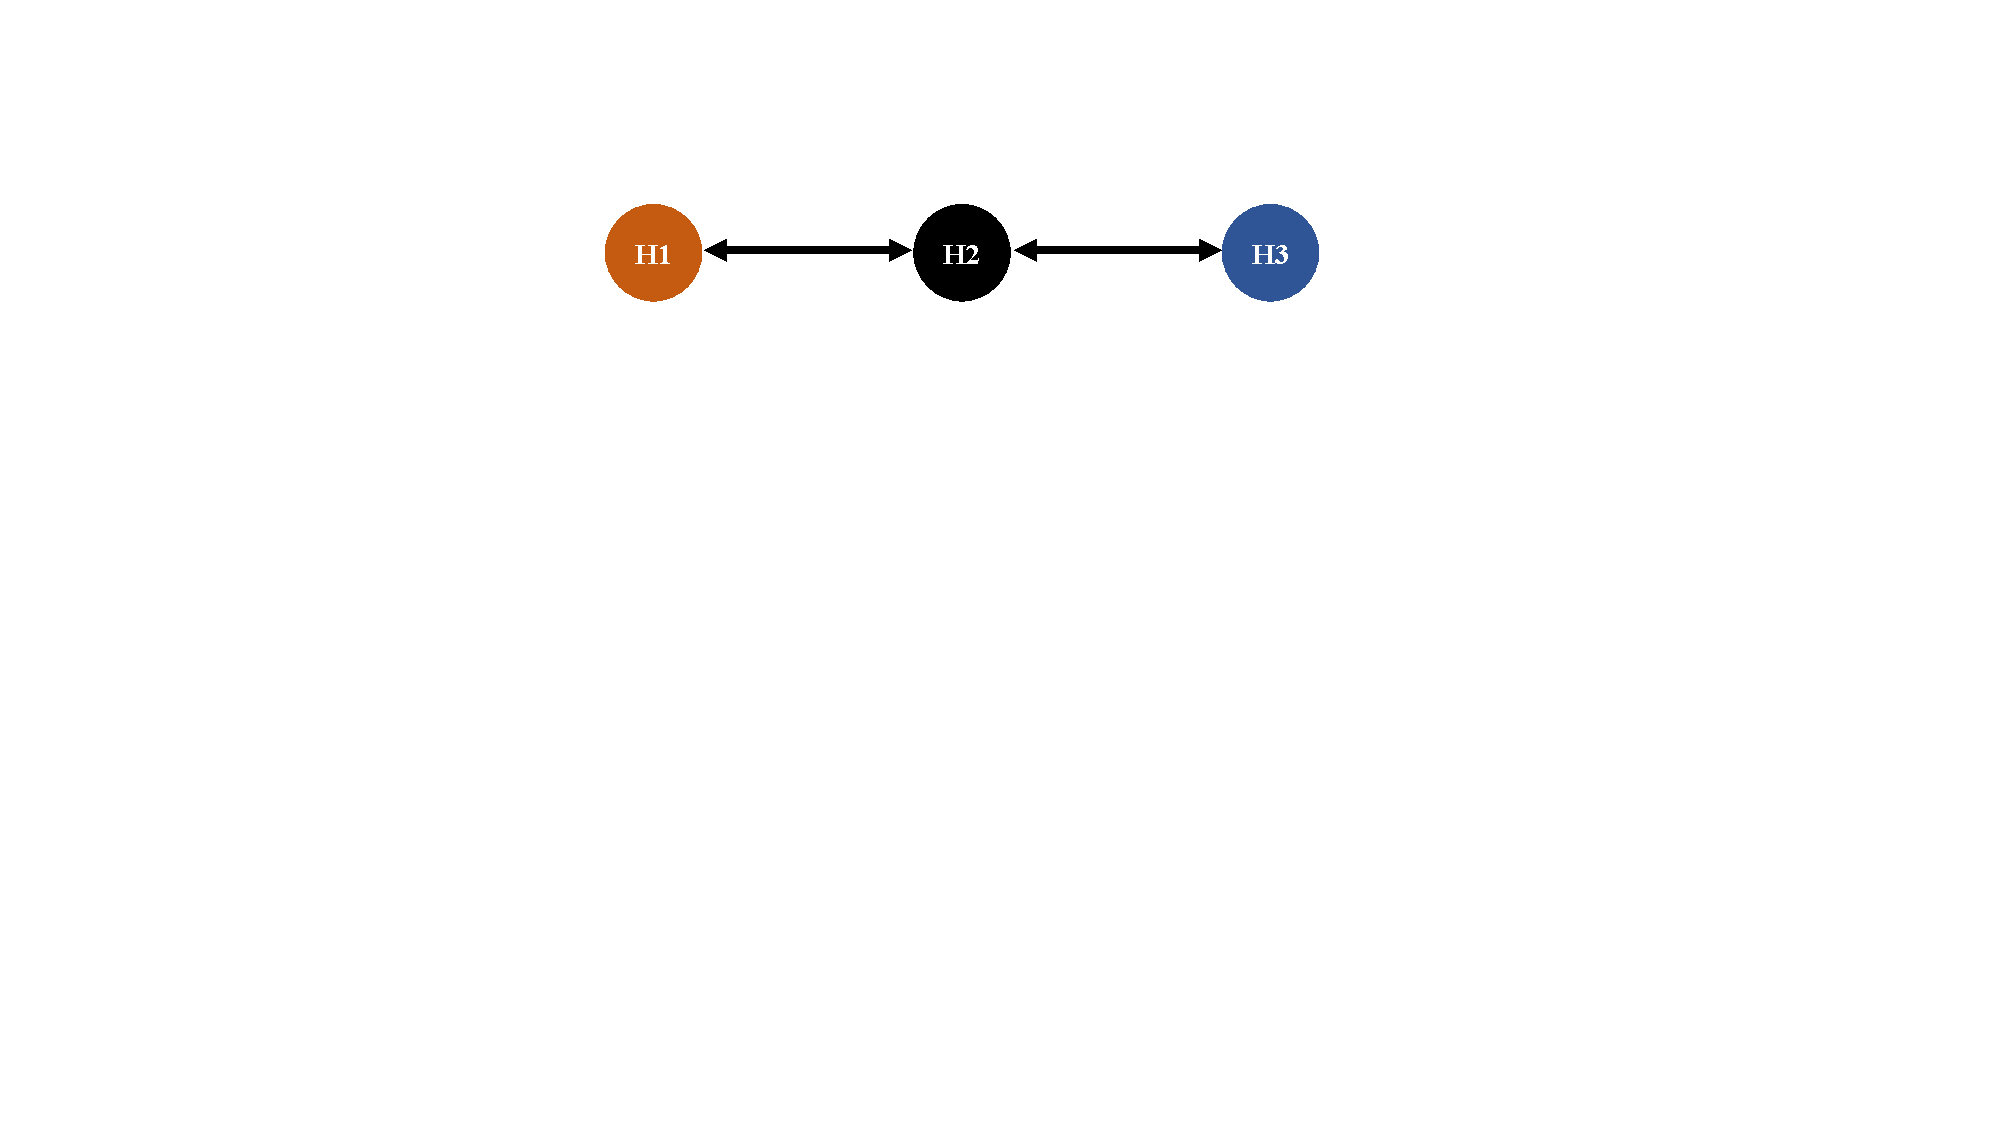
\includegraphics[width=\linewidth]{../figs/Figure_3.pdf}

\begin{itemize}
\item UDP Tunnels \& TCP Tunnels
\item Ethernet \& WiFi
\end{itemize}

\end{frame}


\begin{frame}{Results (WiFi):}

\textbf{UDP (both links):}\\[.3em]
\begin{tabular}{ l r l r }
\toprule
\textbf{Scenario} & \textbf{RTT}	& \textbf{Goodput} & \textbf{Retx} \\
\midrule
Without CC: & 60ms 	& 28.7 Mbps	 & 250 Retx \\
With CC: & 6-9ms 		& 26.0 Mbps		 & 0 Retx \\
\bottomrule
\end{tabular}

\pause
\vspace*{1em}

\textbf{TCP (both links):}\\[.3em]
\begin{tabular}{ l r l r }
\toprule
\textbf{Scenario} & \textbf{RTT}	& \textbf{Goodput} & \textbf{Retx} \\
\midrule
Without CC: & 115ms 	& 37 Mbps	 & 320 Retx \\
With CC: 		& 	7ms  	& 29 Mbps	 & 0 Retx \\
\bottomrule
\end{tabular}

\vspace*{1em}

\pause
Ethernet: Cong. signals can even give you a \textbf{higher goodput!}

\end{frame}


\begin{frame}{Results (WiFi):}

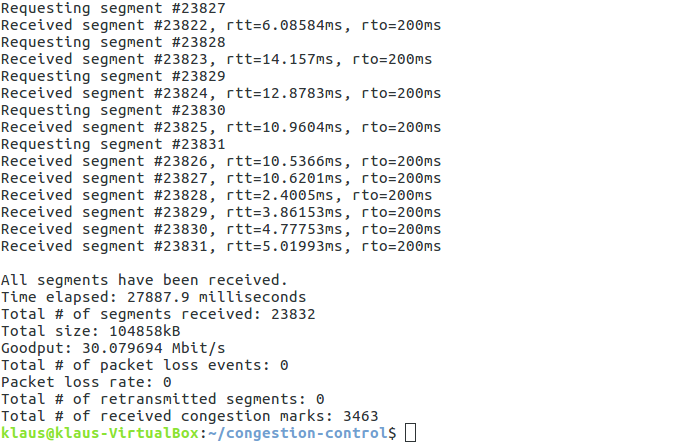
\includegraphics[width=\linewidth]{../results/screenshots.png}

\end{frame}




\begin{frame}{Takeaway:}

{\footnotesize
\url{https://github.com/5th-ndn-hackathon/congestion-control}
}
\begin{enumerate}
\item Congestion detection by socket queue works! 
\item Even works on WiFi (much lower layer).
\item Use UDP Tunnels + congestion signaling everywhere.
\end{enumerate}

\pause
Future work
\begin{enumerate}
\item Implement in NFD (run on testbed)
\item Test ``hidden congestion'' inside IP underlay (tunnel)
\end{enumerate}


\end{frame}




%
%\begin{frame}{Implementation Overview}
%
%From PCON paper \cite{schneider2016practical}:
%	
%	\includegraphics<1>[width=\linewidth]{images/architecture_1.pdf}
%	\includegraphics<2>[width=\linewidth]{images/architecture_2.pdf}
%	\includegraphics<3>[width=\linewidth]{images/architecture_3.pdf}
%	\includegraphics<4>[width=\linewidth]{images/architecture_4.pdf}
%	\includegraphics<5>[width=\linewidth]{images/architecture_5.pdf}
%	
%\end{frame}
%
%\begin{frame}{Implementation Overview: Redmine}
%
%	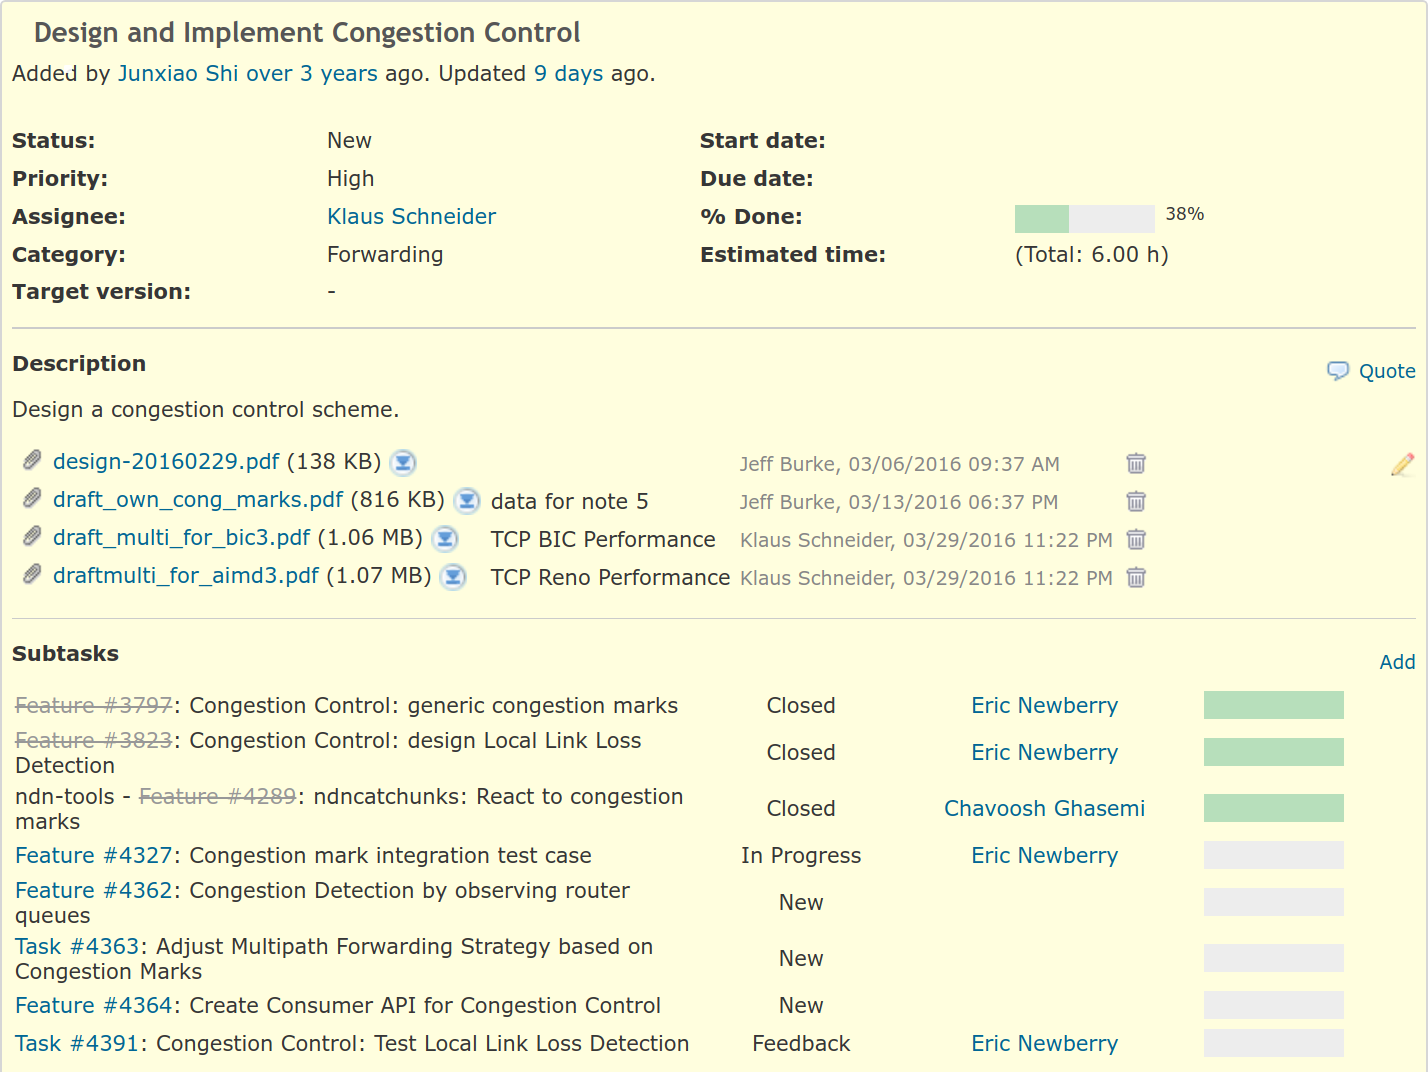
\includegraphics[width=\linewidth]{images/redmine_overview.png}
%
%\end{frame}
%
%\begin{frame}{What We Accomplished since last Retreat}
%	
%	Thanks to Eric, Davide, Chavoosh, Junxiao, and others.
%	\pause
%	\begin{enumerate}
%		\item \textbf{Generic Congestion Marks}
%		\begin{itemize}
%		\item Defined in NDNLP
%		\item Simple API with getters \& setters
%%		to set and get congestion marks.
%		\end{itemize}
%		\pause
%		
%		\item \textbf{Consumer Congestion Adaptation}
%		\begin{itemize}
%		\item Catchunks: AIMD, react to congestion marks
%%		\item Catchunks: AIMD adaptation, reduced version discovery timeout, Conservative (SACK) window adaptation, printSummary
%		\end{itemize}
%		\pause
%		
%		\item \textbf{Local Link Loss Detection} (NDNLP) 
%		\begin{itemize}
%		\item Detect lost packets (via gap in SeqNr or ACK Timeout)
%		\item Signal to forwarding strategy \textbf{onLostInterest()}.
%		\end{itemize}
%	
%	\end{enumerate}
%	
%\end{frame}
%
%
%		% Mark data packets, nacks and Interests
%		%Part of NDNLP
%%		\item Congestion detection on Ethernet links / TCP tunnels?
%%		\begin{itemize}
%%			\item How to get the right queue?
%%			\item How to get the queue inside NFD?
%%%			\item 
%%		\end{itemize}
%%	\item Congestion detection on UDP tunnels %: Detect \& signal link losses
%
%		% How to get 
%
%%\begin{frame}{Congestion detection on UDP tunnels (Testbed)}
%%	Vusirikala et al. -- \textbf{Hop-By-Hop Best Effort Link Layer Reliability in Named Data Networking} (Tech Report)
%%	
%%	Detect local ``link'' losses and signal to forwarding strategy
%%	\pause
%%		\begin{itemize}
%%			\item How many local retransmissions? \pause
%%			\item Decouple loss notification from retx. \pause
%%			\item Positive vs. Negative ACKs? 
%%			\begin{itemize}
%%				\item Definitive knowledge about loss vs. overhead.
%%			\end{itemize}
%%		\pause
%%		
%%			\item ACK duplication?
%%			\begin{itemize}
%%				\item Duplicating ACKs cheaper than spurious retx
%%%				\item 
%%%				\item 
%%			\end{itemize}
%%		\pause
%%		
%%			\item Selective vs. Cumulative ACKs? \pause
%%	\end{itemize}
%%
%%\end{frame}
%
%\begin{frame}{Future Work and Timeline}
%
%\begin{enumerate}
%\item \textbf{Integration tests} (2 months)
%\begin{itemize}
%\item For congestion marks \& link loss detection
%\item Check if current functionality works as expected
%\end{itemize}
%\pause
%\item \textbf{Cong. Detection} based on \textbf{queue backlog}
%(6 months)
%\begin{itemize} 
%%\item Different queues: NIC, kernel, socket queue 
%\item To work on TCP/UDP Tunnels, Ethernet, Wireless
%\item $\Rightarrow$ See our \textbf{Hackathon Project!}
%\end{itemize}
%\pause
%\item \textbf{Consumer/Producer API} (9 months)
%\begin{itemize}
%\item Look at Ilya's work and Cisco's libcnet API
%\end{itemize}
%
%\pause
%\item \textbf{Multipath Forwarding} (needs more design)
%\end{enumerate}
%
%\end{frame}
%
%
%\begin{frame}{Progress in one Picture}
%
%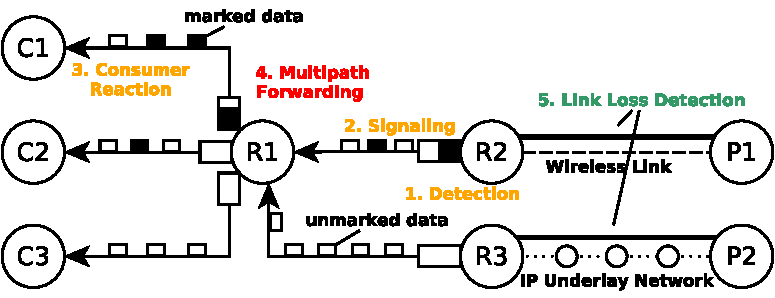
\includegraphics[width=\linewidth]{images/architecture_progress.pdf}
%
%\end{frame}
%
%
%%
%%\begin{frame}{Congestion detection on Ethernet links / TCP tunnels?}
%%	
%%	\begin{enumerate}
%%		\item Ethernet: Read out NIC queue size + apply AQM logic
%%		\item TCP Tunnel: Read send buffer occupancy
%%		%			\item 
%%	\end{enumerate}
%%
%%More work needed:
%%\begin{itemize}
%%		\item How to get the right queue?
%%		\item How to get the queue inside NFD?
%%\end{itemize}
%%	
%%\end{frame}
%%
%%
%%\begin{frame}{More General Questions}
%%	
%%	\begin{itemize}
%%		\item Congestion due to packet processing and memory overhead
%%		\pause
%%		% Wanted functionality? New congestion reaction mechanisms? 
%%		\item DDoS in NDN: A congestion problem? 
%%		\pause
%%		\item BBR's applicability to NDN congestion control
%%%		\item Congestion detection on Ethernet lisnks and on TCP tunnels?
%%		
%%	\end{itemize}
%%	
%%\end{frame}



%% Last slide
\begin{frame}
	\frametitle{The End}
	\vspace{2cm}
	{\huge Any Questions?
%		Thank you for
%		your attention!\\
%		\vspace*{2em}
	}
	\vspace{2.5cm}  
	\begin{flushright}  
		Klaus Schneider, Eric Newberry, Chavoosh Ghasemi \\
%		 \footnotesize{
%%			\url{klaus@cs.arizona.edu} \\
%%			\url{https://www.cs.arizona.edu/~klaus/} %\\ 
%		}
	\end{flushright}
\end{frame}
